% Template created by Karol Kozioł (www.karol-koziol.net) for ShareLaTeX

\documentclass[a4paper,spanish,9pt]{extarticle}
%%%%
\usepackage[T1]{fontenc}
%%%%
\usepackage[utf8]{inputenc}
\usepackage[spanish]{babel}
\usepackage{lmodern}
\usepackage{array}


%\usepackage[T1]{fontenc}
\usepackage{verbatim}
\usepackage{graphicx}
\usepackage{xcolor}
\newcommand{\degre}{\ensuremath{^\circ}}
\usepackage{pgf,tikz,pgfplots}
\usepackage{import}
\pgfplotsset{compat=1.15}
\usetikzlibrary{shapes, calc, shapes, arrows, math, babel, positioning}

\usepackage{amsmath,amssymb,textcomp,mathrsfs}
\everymath{\displaystyle}

\usepackage{times}
\renewcommand\familydefault{\sfdefault}
\usepackage{tgheros}
\usepackage[defaultmono,scale=0.85]{droidmono}

\usepackage{multicol}
\setlength{\columnseprule}{0pt}
\setlength{\columnsep}{20.0pt}

\usepackage[spanish]{babel}
\usepackage{eurosym}


\graphicspath{{./img/}}
%\usepackage{svg}

\usepackage{hyperref}

\usepackage{geometry}
\geometry{
a4paper,
total={210mm,297mm},
left=10mm,right=10mm,top=10mm,bottom=15mm}

\linespread{1.3}

\newcommand{\samedir}{\mathbin{\!/\mkern-5mu/\!}}

% custom title
\makeatletter
\renewcommand*{\maketitle}{%
\noindent
\begin{minipage}{0.6\textwidth}
\begin{tikzpicture}
\node[rectangle,rounded corners=6pt,inner sep=10pt,fill=blue!50!black,text width= 0.95\textwidth] {\color{white}\Huge \@title};
\end{tikzpicture}
\end{minipage}
\hfill
\begin{minipage}{0.35\textwidth}
\begin{tikzpicture}
\node[rectangle,rounded corners=3pt,inner sep=10pt,draw=blue!50!black,text width= 0.95\textwidth] {\begin{tabular}{cc} \multirow{2}{1cm}{
\includegraphics[width=0.15\columnwidth]{header_right}}& \@author \\ & \ies \end{tabular}};
\end{tikzpicture}
\end{minipage}
\bigskip\bigskip
}%
\makeatother

% custom section
\usepackage[explicit]{titlesec}
\newcommand*\sectionlabel{}
\titleformat{\section}
  {\gdef\sectionlabel{}
   \normalfont\sffamily\Large\bfseries\scshape}
  {\gdef\sectionlabel{\thesection\ }}{0pt}
  {
\noindent
\begin{tikzpicture}
\node[rectangle,rounded corners=3pt,inner sep=4pt,fill=blue!50!black,text width= 0.95\columnwidth] {\color{white}\sectionlabel#1};
\end{tikzpicture}
  }
\titlespacing*{\section}{0pt}{15pt}{10pt}


% custom footer
\usepackage{fancyhdr}
\makeatletter
\pagestyle{fancy}
\fancyhead{}
\fancyfoot[C]{\footnotesize \@author \ - \ies}
\renewcommand{\headrulewidth}{0pt}
\renewcommand{\footrulewidth}{0pt}
\makeatother
\usepackage{multirow} % para las tablas


\title{Variables de Probabilidad}
\author{Departamento de Matemáticas}
\date{2014}
\newcommand{\ies}{IES Pedro Cerrada}


\begin{document}

\maketitle



\begin{multicols*}{2}
%
\section{Experimento aleatorio}

Un \textbf{experimento aleatorio} o no determinista es aquél que si se repite varias veces no está garantizado obtener siempre el mismo resultado. Es decir, no se puede determinar cuál va a ser el resultado del experimiento hasta que no se realiza. En caso contrario, decimos que el experimento es \textbf{determinista}

Un experimento es aleatorio cuando depende de muchos factores y cualquier pequeña modificación de alguno implica obtener un resultado diferente.

\subsection{Ejemplos}

\begin{itemize}
 \item \textbf{Aleatorio}: Lanzar un dado y ver el resultado
 \item \textbf{Determinista}: Calcular el tiempo que tarda en caer un objeto al suelo desde una distancia determinada
 \end{itemize} 
 
\section{Espacio muestral y sucesos}
\begin{itemize}
\item \textbf{Espacio muestral}: Conjunto de los posibles resultados del experimento. Se denota: $E$
\item \textbf{Sucesos simples o elementales}: Cualquiera de los elementos del espacio muestral
\item \textbf{Sucesos compuestos}: Sucesos formados por varios simples. 
\item \textbf{Suceso seguro}: Suceso compuesto por los elementos del Espacio muestral. Se cumple siempre
\item \textbf{Suceso imposible}: Cualquier suceso que no se cumpla nunca. Se denota con el símbolo: $\varnothing$
\item \textbf{Suceso contrario}: Si $A$ es un suceso, $\overline{A}$ es el suceso contrario. Es aquel que se cumple cuando no se cumple $A$
\end{itemize}

\subsection{Ejemplo:} Lanzamos un dado y comprobamos la cara que sale.
\begin{itemize}
\item \textbf{Espacio muestral}: $E=\lbrace 1,2,3,4,5,6 \rbrace $
\item \textbf{Sucesos simples o elementales}: $1$, $2$, $3$, $4$, $5$ ó $6$
\item \textbf{Sucesos compuestos}: $A=\lbrace que\ salga\ par\rbrace=\lbrace2,4,6\rbrace$
\item \textbf{Suceso seguro}: $E=\lbrace 1,2,3,4,5,6 \rbrace $
\item \textbf{Suceso imposible}: $\varnothing=\lbrace que\ salga \ mayor \ que \ 6\rbrace$
\item \textbf{Suceso contrario}: Si $A=\lbrace que\ salga\ par\rbrace=\lbrace2,4,6\rbrace$, $\overline{A}=\lbrace que\ salga\ impar\rbrace=\lbrace1,3,5\rbrace$ 
\end{itemize}


\section{Operaciones con sucesos y relaciones}

\def\firstcircle{(0,0) circle (1.5cm)}
\def\secondcircle{(0:2cm) circle (1.5cm)}
\def\espacio{(-2,-2) rectangle (4,2)}

\colorlet{circle edge}{blue!50}
\colorlet{circle area}{blue!20}

\tikzset{filled/.style={fill=circle area, draw=circle edge, thick},
    outline/.style={draw=circle edge, thick}}

\setlength{\parskip}{5mm}
\begin{itemize}
\item \textbf{Unión}: la unión de los sucesos $A$ y $B$ es aquel suceso que contiene a todos los elementos de $A$ y a  los de $B$. Se denota: $A\cup B$ 

% Set A or B
\begin{tikzpicture}[scale=0.8]
\draw[outline] \espacio node[above] {$E$};
    \draw[filled] \firstcircle node {$A$}
                  \secondcircle node {$B$};
    \node[anchor=south] at (1,1.3) {$A \cup B$};
\end{tikzpicture}

\item \textbf{Intersección}: la intersección de los sucesos $A$ y $B$ es aquel suceso que contiene a todos los elementos que están tanto en $A$ como en $B$. Se denota: $A\cap B$ 
 
% Set A and B
\begin{tikzpicture}[scale=0.8]
	\draw[outline] \espacio node[above] {$E$};
    \begin{scope}
        \clip \firstcircle;
        \fill[filled] \secondcircle;
    \end{scope}
    \draw[outline] \firstcircle node {$A$};
    \draw[outline] \secondcircle node {$B$};
    %\node[anchor=south] at (current bounding box.north) {$A \cap B$};
    \node[anchor=south] at (1,1.3) {$A \cap B$};
\end{tikzpicture}
\end{itemize}

\subsection{Ejemplo} Tomamos como experimento el resultado de lanzar un dado, y los sucesos: \\
\begin{tabular}{l}
$A=\lbrace que\ salga\ par\rbrace=\lbrace2,4,6\rbrace$ \\
$B=\lbrace que\ sea\ mayor\ que\ 3\rbrace=\lbrace4,5,6\rbrace$ \\
$C=\lbrace que\ salga\ impar\rbrace=\lbrace1,3,5\rbrace$
\end{tabular}
\begin{itemize}	
	\item $A\cup B=\lbrace2,4,5,6\rbrace$ \\
	% Set A or B
\begin{tikzpicture}[scale=0.7]
\draw[outline] \espacio node[above] {$E$};
    \draw[filled] \firstcircle node[left] {$2$}
                  \secondcircle node[right] {$5$};
    \node[anchor=south] at (1,1.3) {$A \cup B$};
    \node[anchor=south] at (1,0.25) {$4$};
    \node[anchor=south] at (1,-0.75) {$6$};
    
\end{tikzpicture}
	\item $A\cap B=\lbrace4,6\rbrace$\\
	% Set A and B
\begin{tikzpicture}[scale=0.7]
	\draw[outline] \espacio node[above] {$E$};
    \begin{scope}
        \clip \firstcircle;
        \fill[filled] \secondcircle;
    \end{scope}
    \draw[outline] \firstcircle node[left] {$2$};
    \draw[outline] \secondcircle node[right] {$5$};
    %\node[anchor=south] at (current bounding box.north) {$A \cap B$};
    \node[anchor=south] at (1,1.3) {$A \cap B$};
    \node[anchor=south] at (1,0.25) {$4$};
    \node[anchor=south] at (1,-0.75) {$6$};
\end{tikzpicture}
\item $A\cup C=\lbrace1,2,3,4,5,6\rbrace=E$
\item $A\cap C=\varnothing$
\end{itemize}

\subsection{Compatibilidad de sucesos} Se dice que dos sucesos son incompatibles cuando su intersección es el conjunto vacío. En caso contrario se dice que son compatibles.

\subsubsection{Ejemplo} En el ejemplo anterior, $A$ y $B$ son compatibles y $A$ y $C$ incompatibles.


\section{Probabilidad en experimentos regulares y Regla de Laplace} Cuando todos los sucesos elementales de un \textbf{espacio muestral finito} están en las mismas condiciones de suceder se dice que son \textbf{equiprobables}, y al experimento se le llama \textbf{regular}.
\subsection{Ejemplos de experimentos regulares} Lanzamiento de dados, monedas, extracción de cartas, ...

\subsection{Regla de Laplace} La probabilidad de un suceso de un experimento regular viene determinada por la Regla de Laplace:
$$P(A)=\dfrac{Casos\ favorables}{Casos\ posibles} $$
\subsubsection{Ejemplo}
Al lanzar un dado, los casos posibles son 6 ($\lbrace1,2,3,4,5,6\rbrace$):\\
\begin{tabular}{l}
La probabilidad de sacar un 3: $\lbrace3\rbrace\to \dfrac{1}{6}$\\
La probabilidad de sacar par: $\lbrace2,4,6\rbrace\to\dfrac{3}{6}$ \\
La probabilidad de sacar más de 4: $\lbrace5,6\rbrace\to\dfrac{2}{6}$
\end{tabular}

\section{Propiedades de la probabilidad} La probabilidad de un experimento regular cumple las siguientes propiedades:
\begin{itemize}
\item $0 \leq P(A) \leq 1$ 
\item $P(E) = 1$ y $P(\varnothing) = 0$
\item $P(A) + P(\overline A) = 1$
\item $P(A \cup B) = P(A) + P(B) - P(A \cap B)$. Si $A$ y $B$ son icompatibles: $P(A \cup B) = P(A) + P(B)$
\end{itemize}
Podemos extender el concepto de probabilidad a cualquier función que cumpla las propiedades anteriores.  

\section{Probabilidad condicionada}

Puesto que la probabilidad está ligada al nivel de confianza sobre los resultados de un experimento, el hecho de que ocurra un suceso, puede cambiar la probabilidad de los demás. A esta nueva probabilidad se le llama \textbf{condicionada}
\subsection{Ejemplo}
 Supongamos que tenemos una urna con 8 bolas numeradas pero de colores blancos y negros de la cual se extrae una. Supongamos, también, que las tres primeras son blancas y el resto negras, luego  $E=\lbrace B_1,B_2, B_3, N_4, N_5, N_6, N_7, N_8\rbrace$.\\
 A priori, la $P(\lbrace Sea\ impar\rbrace )=\frac{4}{8}=\frac{1}{2}$ por la regla de Laplace. Tiene la misma probabilidad salir par que impar\\
 Vamos a suponer ahora que durante la extracción se percibe que la bola es blanca. La situación cambia, porque que sea blanca implica que hay 3 casos posibles y dos de las tres son impares. A esta nueva probabilidad se le llama  condicionada y se denota así:
 $$P(I|B)=\dfrac{2}{3}$$
La probabilidad de que sea impar ha aumentado por el hecho de haber añadido la condición (o información) que es blanca.\\
Esta probabilidad la podemos transformar:
 $$P(I|B)=\dfrac{2}{3}=\dfrac{\dfrac{2}{8}}{\dfrac{3}{8}}=\dfrac{P(I\cap B)}{P(B)}$$

\subsection{Generalización del fórmula de la probabilidad condicionada} $$P(A|B)=\dfrac{P(A\cap B)}{P(B)}$$
y despejando:
$$P(A\cap B) = P(A|B)\cdot P(B)$$

\section{Experimentos compuestos} Un \textbf{experimento aleatorio compuesto} es el que está formado por varios experimentos simples realizados de forma consecutiva.
\subparagraph{Ejemplo:}Lanzar tre monedas, extraer cuatro cartas de una baraja, ...

La probabilidad de un suceso compuesto se podrá calcular a partir de las probabilidades obtenidas de los experimentos simples usando la probabilidad condicional:
$$P(A\cap B) = P(A) \cdot P(B|A)$$

\subsection{Independencia y dependencia de sucesos}
Se dice que dos sucesos son independientes cuando la probabilidad de cada uno no depende del resultado del otro. 

$$A\ y \ B\ son \ independientes \Longleftrightarrow P(B|A)=P(B)$$

\subparagraph{Ejemplos de sucesos independientes:}  Lanzar varias monedas, extracción de varias cartas con reemplazamiento, sacar bolas de una urna con reemplazamiento, lanzar varios dados, ...
\subparagraph{Ejemplos de sucesos dependientes:}  Extracción de varias cartas sin reemplazamiento, sacar bolas de una urna sin reemplazamiento, ...

\subsection{Cálculo de probabilidad compuesta para sucesos dependientes}
\paragraph{Ejemplo:} En una urna hay tres bolas blancas y dos negras. Se extraen dos bolas \textbf{sin} reemplazamiento. Podemos construir el siguiente árbol con las probabilidades de los diferentes resultados:

\tikzstyle{bag} = [text width=4em, text centered]
\tikzstyle{end} = [circle, minimum width=3pt,fill, inner sep=0pt]
\tikzstyle{level 1} = [level distance=3.5cm, sibling distance=3.5cm]
\tikzstyle{level 2} = [level distance=3.5cm, sibling distance=2cm]
\begin{tikzpicture}[grow=right, sloped, scale=0.7]
\node[bag] {$3_B, 2_N$}
    child {
        node[bag] {$3_B, 1_N$}        
            child {
                node[end, label=right:
                    {$P(N_1\cap N_2)=\frac{2}{5}\cdot\frac{1}{4}$}] {}
                edge from parent
                node[above] {$N$}
                node[below]  {$1/4$}
            }
            child {
                node[end, label=right:
                    {$P(N_1\cap B_2)=\frac{2}{5}\cdot\frac{3}{4}$}] {}
                edge from parent
                node[above] {$B$}
                node[below] {$3/4$}
            }
            edge from parent 
            node[above] {$N$}
            node[below]  {$2/5$}
    }
    child {
        node[bag] {$2_B, 2_N$}        
        child {
                node[end, label=right:
                    {$P(B_1\cap N_2)=\frac{3}{5}\cdot\frac{2}{4}$}] {}
                edge from parent
                node[above] {$N$}
                node[below]  {$2/4$}
            }
            child {
                node[end, label=right:
                    {$P(B_1\cap B_2)=\frac{3}{5}\cdot\frac{2}{4}$}] {}
                edge from parent
                node[above] {$B$}
                node[below]  {$2/4$}
            }
        edge from parent         
            node[above] {$B$}
            node[below]  {$3/5$}
    };
\end{tikzpicture} \\
\subparagraph{Ejemplos:}\begin{list}{-}{}
\item Probabilidad de que las dos sean blancas:\\
$P(B_1\cap B_2)=P(B_1)\cdot P(B_2|B_1)=\frac{3}{5}\cdot\frac{2}{4}=\frac{3}{10}$
\item Probabilidad de que las dos sean negras:\\ 
$P(N_1\cap N_2)=P(N_1)\cdot P(N_2|N_1)=\frac{2}{5}\cdot\frac{1}{4}=\frac{1}{10}$
\item Probabilidad de que sean del mismo color: \\
$P((B_1\cap B_2)\cup (N_1\cap N_2))=\frac{3}{10}+\frac{1}{10}=\frac{2}{5}$
\end{list}


\subsection{Cálculo de probabilidad compuesta para sucesos independientes}
\paragraph{Ejemplo:} En una urna hay tres bolas blancas y dos negras. Se extraen dos bolas \textbf{con} reemplazamiento. Ahora el árbol quedará:\\
\begin{tikzpicture}[grow=right, sloped, scale=0.7]
\node[bag] {$3_B, 2_N$}
    child {
        node[bag] {$3_B, 2_N$}        
            child {
                node[end, label=right:
                    {$P(N_1\cap N_2)=\frac{2}{5}\cdot\frac{2}{5}$}] {}
                edge from parent
                node[above] {$N$}
                node[below]  {$2/5$}
            }
            child {
                node[end, label=right:
                    {$P(N_1\cap B_2)=\frac{2}{5}\cdot\frac{3}{5}$}] {}
                edge from parent
                node[above] {$B$}
                node[below] {$3/5$}
            }
            edge from parent 
            node[above] {$N$}
            node[below]  {$2/5$}
    }
    child {
        node[bag] {$3_B, 2_N$}        
        child {
                node[end, label=right:
                    {$P(B_1\cap N_2)=\frac{3}{5}\cdot\frac{2}{5}$}] {}
                edge from parent
                node[above] {$N$}
                node[below]  {$2/5$}
            }
            child {
                node[end, label=right:
                    {$P(B_1\cap B_2)=\frac{3}{5}\cdot\frac{3}{5}$}] {}
                edge from parent
                node[above] {$B$}
                node[below]  {$3/5$}
            }
        edge from parent         
            node[above] {$B$}
            node[below]  {$3/5$}
    };
\end{tikzpicture} \\
\subparagraph{Ejemplos:}\begin{list}{-}{}
\item Probabilidad de que las dos sean blancas:\\
$P(B_1\cap B_2)=P(B_1)\cdot P(B_2|B_1)=\frac{3}{5}\cdot\frac{3}{5}=\frac{9}{25}$
\item Probabilidad de que las dos sean negras:\\ 
$P(N_1\cap N_2)=P(N_1)\cdot P(N_2|N_1)=\frac{2}{5}\cdot\frac{2}{5}=\frac{4}{25}$
\item Probabilidad de que sean del mismo color: \\
$P((B_1\cap B_2)\cup (N_1\cap N_2))=\frac{9}{25}+\frac{4}{25}=\frac{13}{25}$
\end{list}


\section{Teorema de la probabilidad total}
\paragraph{Ejemplo:} En un instituto de ESO hay 4 cursos: 1º, 2º, 3º y 4º. Se quiere estudiar la probabilidad de que un alumno del instituto esté con la gripe (Llamamos $G$ al suceso tener gripe). 

\begin{tikzpicture}
\tikzset{
    myrectangle/.style={
        draw=black,
        minimum width=4cm,
        minimum height=2cm,
    },
    B/.style={
        draw=blue,
    },
    A/.style={
        draw=green,
    },
    >=stealth,
    node distance=1cm and 1cm,
}

    \node[myrectangle] (left) {};
    \node[myrectangle] (right) [right=of left] {};
    \path (left.south east) -- coordinate (tmp) (right.south west);
    \node[myrectangle] (bottom) [below=of tmp] {};

    % "contents" of left node
    \path (left.north west) -- node[pos=.5] {$ESO_1$} (left.center);
    \path (left.north east) -- node[pos=.5] {$ESO_2$} (left.center);    
    \path (left.south west) -- node[pos=.5] {$ESO_3$} (left.center);
    \path (left.south east) -- node[pos=.5] {$ESO_4$} (left.center);
    
    
    
\draw[B] ($(left.north west) ! .5 ! (left.north east)$) -- ($(left.south west) ! .5 ! (left.south east)$);

\draw[B] ($(left.north west) ! .5 ! (left.south west)$) -- ($(left.north east) ! .5 ! (left.south east)$);


    % "contents" of right node
    \draw[A] (right.center) ellipse [x radius=1.3cm, y radius=.7cm] node {$G$};

    % "contents" of bottom node
    \path (bottom.north west) -- node[pos=.73] {$G\cap E_1$} (bottom.center);
    \path (bottom.north east) -- node[pos=.73] {$G\cap E_2$} (bottom.center);    
    \path (bottom.south west) -- node[pos=.73] {$G\cap E_3$} (bottom.center);
    \path (bottom.south east) -- node[pos=.73] {$G\cap E_4$} (bottom.center);

\draw[B] ($(bottom.north west) ! .5 ! (bottom.north east)$) -- ($(bottom.south west) ! .5 ! (bottom.south east)$);

\draw[B] ($(bottom.north west) ! .5 ! (bottom.south west)$) -- ($(bottom.north east) ! .5 ! (bottom.south east)$);

    \draw[A] (bottom.center) ellipse [x radius=1.3cm, y radius=.7cm];

    % arrows
    \begin{scope}[
        shorten >=.2cm,
        shorten <=.2cm,
    ]
        \draw[->, black] (left) -- (bottom);
        \draw[->, black] (right) -- (bottom);
    \end{scope}

    % labels on top
    \node at (left.north east) [anchor=south east] {E};
    \node at (right.north east) [anchor=south east] {E};
    \node at (bottom.north east) [anchor=south east] {E};

\end{tikzpicture}

Como un alumno pertenece a un solo curso los sucesos $ESO_1$ , $ESO_2$, $ESO_3$, y $ESO_4$ (abreviados $E_1$, etc.) son incompatibles. Además: $$G=(G \cap E_1)\cup(G \cap E_2)\cup(G \cap E_3)\cup(G \cap E_4)=\bigcup_{i=1}^4(G \cap E_i)$$
Por tanto,
$$P(G)=P(G \cap E_1)+P(G \cap E_2)+P(G \cap E_3)+P(G \cap E_4)=\sum_{i=1}^4 P(G \cap E_i)$$
Aplicando la probabilidad condicionada:
\begin{eqnarray*}
P(G)=P(E_1)\cdot P(G|E_1)+P(E_2)\cdot P(G|E_2)+\\+P(E_3)\cdot P(G|E_3)+P(E_1)\cdot P(G|E_4)= \\ =\sum_{i=1}^4 P(E_i)\cdot  P(G|E_i)
\end{eqnarray*}

\subsection{Probabilidad total}
Generalizando el resultado anterior:

\paragraph{Teorema de la probabilidad total:} Si $A_1$, $A_2$, ..., $A_n$   son sucesos incompatibles dos a dos y cuya unión es todo el espacio muestral, entonces la probabilidad de cualquier otro suceso $B$ es:

$$P(B)=\sum_{i=1}^n P(A_i)\cdot  P(B|A_i) $$

\subsubsection{Ejemplo:} Tomando de nuevo el ejemplo de la urna en la que hay tres bolas blancas y dos negras. Si se extraen dos bolas, por ejemplo \textbf{sin} reemplazamiento, podemos calcular la probabilidad de que la segunda bola haya sido blanca: 

\tikzstyle{bag} = [text width=4em, text centered]
\tikzstyle{end} = [circle, minimum width=3pt,fill, inner sep=0pt]
\tikzstyle{level 1} = [level distance=3.5cm, sibling distance=3.5cm]
\tikzstyle{level 2} = [level distance=3.5cm, sibling distance=2cm]
\begin{tikzpicture}[grow=right, sloped, scale=0.7]
\node[bag] {$3_B, 2_N$}
    child {
        node[bag] {$3_B, 1_N$}        
            child {
                node[end, label=right:
                    {$P(N_1\cap N_2)=\frac{2}{5}\cdot\frac{1}{4}$}] {}
                edge from parent
                node[above] {$N$}
                node[below]  {$1/4$}
            }
            child {
                node[end, label=right:
                    {$P(N_1\cap B_2)=\frac{2}{5}\cdot\frac{3}{4}$}] {}
                edge from parent
                node[above] {$B$}
                node[below] {$3/4$}
            }
            edge from parent 
            node[above] {$N$}
            node[below]  {$2/5$}
    }
    child {
        node[bag] {$2_B, 2_N$}        
        child {
                node[end, label=right:
                    {$P(B_1\cap N_2)=\frac{3}{5}\cdot\frac{2}{4}$}] {}
                edge from parent
                node[above] {$N$}
                node[below]  {$2/4$}
            }
            child {
                node[end, label=right:
                    {$P(B_1\cap B_2)=\frac{3}{5}\cdot\frac{2}{4}$}] {}
                edge from parent
                node[above] {$B$}
                node[below]  {$2/4$}
            }
        edge from parent         
            node[above] {$B$}
            node[below]  {$3/5$}
    };
\end{tikzpicture}
$$P(B_2)=P(B_1)\cdot P(B_2|B_1) + P(N_1)\cdot P(B_2|N_1)
= \frac{3}{5}\cdot\frac{2}{4} + \frac{2}{5}\cdot\frac{3}{4}$$

\section{Teorema de Bayes}

Si $A_1$, $A_2$, ..., $A_n$   son sucesos incompatibles dos a dos y cuya unión es todo el espacio muestral, y $B$ otro suceso cualquiera:

$$P(A_i|B)=\dfrac{P(A_i \cap B)}{\sum_{i=1}^n P(A_i)\cdot  P(B|A_i)} $$

\paragraph{Demostración:} Por la probabilidad condicionada:
$$P(A_i|B)=\dfrac{P(A_i \cap B)}{P(B)} $$
Pero por la probabilidad total:
$$P(B)=\sum_{i=1}^n P(A_i)\cdot  P(B|A_i)$$
Sustituyendo esta en la primera obtenemos el resultado
\subsection{Ejemplo:} En el ejemplo del apartado anterior calcular la probabilidad de que la primera bola haya sido blanca si se sabe que la segunda ha sido blanca:
$$P(B_1|B_2)=\dfrac{P(B_1 \cap B_2)}{P(B_1)\cdot  P(B_2|B_1)+P(N_1)\cdot  P(N_2|B_1)}=\dfrac{\dfrac{3}{5}\cdot\dfrac{2}{4}}{\dfrac{3}{5}\cdot\dfrac{2}{4} + \dfrac{2}{5}\cdot\dfrac{3}{4}}$$





\section{Variables aleatorias y distribuciones de probabilidad}

\paragraph{Finalidad :} Abstraer matemáticamente un tipo de experimento aleatorio. Y, con ello, poder estimar de manera teórica lo que sucedería de manera experimental mediante una estadística. 

\paragraph{¿Cómo?:} Mediante variables aleatorias y distribuciones de probabilidad asociadas a esas variables:

\section{Variables aleatorias} Una variable aleatoria es una función que a cada suceso
elemental de un espacio muestral le asigna un número. Para hacer referencia a las variables se usan las letras: $X$, $Y$, ...

\paragraph{Ejemplo:} Sea el experimento aleatorio “lanzar un dado”: El espacio muestral lo componen las 6 caras del dado. Podemos asignar la variable $X$ que a cada cara le asocia el número que represente su cara.

\begin{center}
\begin{tabular}{ccc}
 & $X$ &  \\
Suceso &  &  $x_i$\\ \hline 
Cara 1 & $\rightarrow$ & 1 \\ 
Cara 2 & $\rightarrow$ & 2 \\ 
Cara 3 & $\rightarrow$ & 3 \\ 
Cara 4 & $\rightarrow$ & 4 \\ 
Cara 5 & $\rightarrow$ & 5 \\ 
Cara 6 & $\rightarrow$ & 6 \\ 
\end{tabular} 
\end{center}

\paragraph{Ejemplo:} Sea el experimento compuesto lanzar dos monedas. Podemos asignar la variable aleatoria: $$Y=\left\lbrace Número \ de \ caras \right\rbrace$$

\begin{center}
\begin{tabular}{ccc}
 & $Y$ &  \\
Suceso &  &  $y_i$\\ \hline 
C,C & $\rightarrow$ & 2 \\ 
C,X & $\rightarrow$ & 1 \\ 
X,C & $\rightarrow$ & 1 \\ 
X,X & $\rightarrow$ & 0 \\ 
\end{tabular} 
\end{center}

\subsection{Tipos de variables aleatorias}
\begin{description}
\item[Discretas:] Toman un número finito o numerable de valores
\item[Continuas:] Toman valores en un rango continuo
\end{description}

\paragraph{Ejemplo de variables discreta:} Sea la \emph{X =“El número de caras al lanzar dos dados”}. Los valores posibles son 0, 1 o 2 (que es un conjunto finito de datos, en concreto 3 datos) 

\paragraph{Ejemplo de variables continua:} \emph{X = “Distancia al centro de la diana medida desde la posición en que cae un dardo lanzado por un tirador experto” }. En este caso la variable puede tomar cualquier valor en el rango entre 0 y el radio de la diana 

\section{Distribuciones de probabilidad}

Llamaremos Distribución de probabilidad a la relación entre los valores de la variable y sus probabilidades.

Estas relaciones se pueden indicar mediante el uso de funciones. El tipo de función y su tratamiento es diferente según las variables sean discretas o continuas.

Veamos algunas distribuciones:


\section{Distribución uniforme discreta}

\paragraph{Ejemplo: } Sea la variable \emph{X = “Número obtenido al lanzar una dado”}\\
A cada valor de la variable podemos asignarle su probabilidad:

%\begin{center}
%\begin{tabular}{ccc}
% & $P(X)$ &  \\
%Suceso &  &  $y_i$ \\ \hline 
%1 & $\rightarrow$ & \frac{1}{6} \\ 
%2 & $\rightarrow$ & \frac{1}{6} \\ 
%3 & $\rightarrow$ & \frac{1}{6} \\ 
%4 & $\rightarrow$ & \frac{1}{6} \\ 
%5 & $\rightarrow$ & \frac{1}{6} \\ 
%6 & $\rightarrow$ & \frac{1}{6} \\ 
%\end{tabular} 
%\end{center}

\begin{center}
\begin{tabular}{ccc}
 & $P(X)$ &  \\
$x_i$ &  &  $P(x_i)$\\ \hline 
1 & $\rightarrow$ & $\tfrac{1}{6}$ \\ 
2 & $\rightarrow$ & $\tfrac{1}{6}$ \\ 
3 & $\rightarrow$ & $\tfrac{1}{6}$ \\ 
4 & $\rightarrow$ & $\tfrac{1}{6}$ \\ 
5 & $\rightarrow$ & $\tfrac{1}{6}$ \\ 
6 & $\rightarrow$ & $\tfrac{1}{6}$ \\ 
\end{tabular} 
\end{center}

Podemos representar la relación anterior mediante una función:

%$$f\colon \begin{array}{lc} 
%         & X \rightarrow Y \\ 
%         & x \mapsto f(x)=\frac{x-1}{2} 
%         \end{array}$$
%
%
%$$f\colon \begin{array}{>{\displaystyle}l} 
%          X \rightarrow Y \\ 
%          x\mapsto f(x)=\frac{x-1}{2} 
%         \end{array}$$

$$P\colon \begin{array}{ll} 
          X \rightarrow \mathbb{R} \\ 
          x_i\mapsto P(X=x_i)=\frac{1}{n} 
         \end{array}$$

Todas las caras tienen la misma probabilidad: $\frac{1}{n}$, siendo $n$ el número de caras, o tamaño del espacio muestral. 

A este tipo de distribución se le llama \textbf{uniforme discreta}.

\section{Distribución Binomial}

\paragraph{Ejemplo:} Queremos calcular las probabilidades de que al lanzar 5 monedas, obtengamos tres caras.
Un suceso que cumple el enunciado es:
$$S_1=\left\lbrace C,C,C,X,X \right\rbrace$$
Teniendo en cuenta que lanzar cada moneda son experimentos independientes, la probabilidad de ese suceso será:
%$$P\left(S_1\right)=P\left(C_1\right)\cdot P\left(C_2 C_1 \right)$$
\begin{eqnarray*}
P\left(S_1\right) & = &P\left(C_1\right)\cdot P\left(C_2 | C_1 \right)\cdot ... \cdot P\left(X_5 | C_1 \cap C_2  \cap C_3  \cap X_4   \right)= \\ &  = & P\left(C_1\right)\cdot  P\left(C_2\right) \cdot P\left(C_3\right) \cdot P\left(X_4\right) \cdot P\left(X_5\right)= \\
& = & P\left(C\right)^3\cdot  P\left(X\right)^2
\end{eqnarray*}

Como la probabilidad de que una moneda sea cara es $\frac{1}{2}$ y la de que sea cruz también:

$$P\left(S_1\right)=\left(\frac{1}{2}\right)^3\cdot  \left(\frac{1}{2}\right)^2$$

Ahora bien, habrá tantos sucesos que cumplan el enunciado como combinaciones de 5 elementos tomados de 3 en 3. Por tanto la probabilidad de que salgan 3 caras será:

$$P\left(Salgan \ 3 \ caras\right)=\binom{5}{3}\left(\frac{1}{2}\right)^3\cdot  \left(\frac{1}{2}\right)^2$$

Si asociamos al experimento "lanzar 5 monedas" le asignamos la variable "número de caras obtenidas", podemos determinar la probabilidad mediante la siguiente función.

$$P\colon \begin{array}{l} 
          X \rightarrow \mathbb{R} \\ 
          k\mapsto P(X=k)=\binom{5}{k}\left(\frac{1}{2}\right)^k\cdot  \left(\frac{1}{2}\right)^{5-k} 
         \end{array}$$

Esto es un ejemplo de distribución binomial de tamaño $5$ y probabilidad $0.5$ .

Realizando los cálculos para $k = 1,...,5 $, la distribución de probabilidad de $X$ que resulta es:

\begin{center}
\begin{tabular}{ccc}
 & $P(X)$ &  \\
$x_i$ &  &  $P(x_i)$\\ \hline 
0 & $\rightarrow$ & $0.03125$ \\ 
1 & $\rightarrow$ & $0.15625$ \\ 
2 & $\rightarrow$ & $0.3125$ \\ 
3 & $\rightarrow$ & $0.3125$ \\ 
4 & $\rightarrow$ & $0.15625$ \\ 
5 & $\rightarrow$ & $0.03125$ \\ 
\end{tabular} 
\end{center}

Y gráficamente: 

%\documentclass{article}
%\usepackage{pgfplots}
%\pgfplotsset{compat=1.7}
%
%\begin{document}
\begin{tikzpicture}[
    declare function={binom(\k,\n,\p)=\n!/(\k!*(\n-\k)!)*\p^\k*(1-\p)^(\n-\k);}
]
\begin{axis}[
    samples at={0,...,5},
    yticklabel style={
        /pgf/number format/fixed,
        /pgf/number format/fixed zerofill,
        /pgf/number format/precision=1
    },
    ybar=0pt, bar width=1
]
\addplot [fill=cyan, fill opacity=0.5] {binom(x,5,0.5)}; \addlegendentry{$p=0.5$}

\end{axis}
\end{tikzpicture}
%\end{document}


\paragraph{Generalización de distribución Binomial:} Hablaremos de una distribución binomial cuando:
\begin{itemize}
\item Se parte de un experimento compuesto de varios simples independientes
\item Los experimentos simples son dicotómicos. Es decir, solo puede haber dos sucesos elementales: uno al que llamaremos acierto y otro al que llamaremos fracaso
\item Asociado al experimento compuesto tenemos la variable número de aciertos cuando realizamos el experimento simple un número determinado de veces
\end{itemize}

En la situación anterior, la distribución binomial vendrá determinada por dos parámetros:
\begin{itemize}
\item Parámetro $n$: Número de veces que se realiza el experimento simple 
\item Parámetro $p$: La probabilidad de que ocurra el suceso acierto
\end{itemize}


A este tipo de variable y su distribución de probabilidades se le llama binomial. \\


\paragraph{Ejemplo:} Así en el ejemplo de las monedas, el experimento se compone de \textbf{5 lanzamientos de moneda}. Si sale cara es acierto y si no fracaso. La variable aleatoria asociada al experimento será el número de caras que salen al lanzar 5 monedas. Esta variable sigue una distribución binomial.

\subsection{Probabilidad de la binomial}\textbf{En general tendremos una binomial de tamaño $n$ y probabilidad $p$}, cuando el experimento simple se haga $n$ veces y la probabilidad de acierto sea $p$.

La función de probabilidad en este caso nos queda:
 
 $$P\colon \begin{array}{l} 
          X \rightarrow \mathbb{R} \\ 
          k\mapsto P(X=k)=\binom{n}{k}\left(p\right)^k\cdot  \left(1-p\right)^{n-k} 
         \end{array}$$
         
\paragraph{Ejemplos:} Representación gráfica de algunas binomiales:    
         
%\documentclass{article}
%\usepackage{pgfplots}
%
%\begin{document}
\begin{tikzpicture}[
    declare function={binom(\k,\n,\p)=\n!/(\k!*(\n-\k)!)*\p^\k*(1-\p)^(\n-\k);}
]
\begin{axis}[
    samples at={0,...,40},
    yticklabel style={
        /pgf/number format/fixed,
        /pgf/number format/fixed zerofill,
        /pgf/number format/precision=1
    }
]
\addplot [only marks, cyan] {binom(x,40,0.2)}; \addlegendentry{$p=0.2 \, n=40$}
\addplot [only marks, orange] {binom(x,40,0.5)}; \addlegendentry{$p=0.5 \, n=40 $}
\end{axis}
\end{tikzpicture}
%\end{document}
         
 

\section{Distribución Normal}
Se trata de una distribución asociada a a un variable continua. Tiene dos parámetros:
\begin{itemize}
    \item $\mu :$ Media de la distribución
    \item $\sigma :$ Desviación típica
\end{itemize}
Y se denota así: $
X \sim \mathcal{N}(\mu,\,\sigma)\,.
    $ 
    
La probabilidad total es 1 y la variable $X$ puede tomar $\infty$ valores ($x \in \left(-\infty, +\infty\right)$). Por tanto, en variables continuas la probabilidad de que tome un valor concreto será 0 ($\lim_{x \to \infty}\frac{1}{x}=0$).    

\subsection{función de densidad de una variable continua:}  En variables continuas solo tiene sentido calcular la probabilidad en intervalos.
Se llama \textbf{función de densidad} ($f(x)$) aquella que: 

$$P\left(a\leq X \leq b \right) = \int_{a}^{b} f(x) dx$$

La interpretación gráfica de lo anterior nos dice que la probabilidad de un intervalo corresponde con el área de la función de densidad en ese intervalo.

%\documentclass{article}
%\usepackage{pgfplots}
%\usetikzlibrary{math}
%\begin{document}



\begin{tikzpicture}[scale=0.7]

\pgfmathdeclarefunction{gauss}{2}{%
  \pgfmathparse{1/(#2*sqrt(2*pi))*exp(-((x-#1)^2)/(2*#2^2))}%
}

\tikzmath{
			\conf = 0.96; \crit= 2.05; \a=round(1-\conf)/2,2);
          }

%\begin{axis}[
%  no markers, domain=0:10, samples=100,
%  axis lines*=left, xlabel=$x$, ylabel=$y$,
%  every axis y label/.style={at=(current axis.above origin),anchor=south},
%  every axis x label/.style={at=(current axis.right of origin),anchor=west},
%  height=5cm, width=12cm,
%  xtick={4,6.5}, ytick=\empty,
%  enlargelimits=false, clip=false, axis on top,
%  grid = major
%  ]
%  \addplot [fill=cyan!20, draw=none, domain=0:5.96] {gauss(6.5,1)} \closedcycle;
%  \addplot [very thick,cyan!50!black] {gauss(4,1)};
%  \addplot [very thick,cyan!50!black] {gauss(6.5,1)};
%
%
%%\draw [yshift=-0.6cm, latex-latex](axis cs:4,0) -- node [fill=white] {$1.96\sigma$} (axis cs:5.96,0);
%\end{axis}

\begin{axis}[
  no markers, domain=-5:5, samples=100,
  axis lines=left, 
  %xlabel=$xa$, ylabel=$ya$,
  %every axis y label/.style={at=(current axis.above origin),anchor=south},
  %every axis x label/.style={at=(current axis.right of origin),anchor=west},
  height=5cm, width=12cm,
  xtick={-1,\crit}, ytick=\empty,
  xticklabels = {$a$, $b$},
  enlargelimits=false, clip=false, axis on top,
  %grid = major
  ]
  \addplot [fill=cyan!20, draw=none, domain=-1:\crit] {gauss(0,1)} \closedcycle;
  \addplot [very thick,cyan!50!black] {gauss(0,1)};
  %\addplot [very thick,cyan!50!black] {gauss(6.5,1)};
  


%\draw [yshift=-0.6cm, latex-latex](axis cs:4,0) -- node [fill=white] {$1.96\sigma$} (axis cs:5.96,0);
\end{axis}
\node[] at (5.5,1.5) {$P\left(a\leq X \leq b \right) $};	




\end{tikzpicture}

%\end{document}

\subsection{función de densidad de una distribución normal:}  En el caso de una $
X \sim \mathcal{N}(\mu,\,\sigma)
    $, la función de densidad es:
    $$f(x)=\frac{1}{{\sigma \sqrt {2\pi } }}e^{{{ - \left( {x - \mu } \right)^2 } \mathord{\left/ {\vphantom {{ - \left( {x - \mu } \right)^2 } {2\sigma ^2 }}} \right. \kern-\nulldelimiterspace} {2\sigma ^2 }}}$$
\paragraph{Ejemplos de representaciones gráficas de normales:} 
%\documentclass{article}
%\usepackage{pgfplots}
%\begin{document}



\begin{tikzpicture}
\pgfmathdeclarefunction{gauss}{2}{%
  \pgfmathparse{1/(#2*sqrt(2*pi))*exp(-((x-#1)^2)/(2*#2^2))}%
}

\begin{axis}[every axis plot post/.append style={
  mark=none,domain=-2:3,samples=50,smooth}, % All plots: from -2:2, 50 samples, smooth, no marks
  axis x line*=bottom, % no box around the plot, only x and y axis
  axis y line*=left, % the * suppresses the arrow tips
  enlargelimits=upper] % extend the axes a bit to the right and top
  \addplot {gauss(0,0.5)};
  \addlegendentry{$\mu=0 \land \sigma^{2}=0.5$}
  \addplot {gauss(1,0.75)};
  \addlegendentry{$\mu=1 \land \sigma^{2}=0.75$}
  \addplot {gauss(0,1)};
  \addlegendentry{$\mu=0 \land \sigma^{2}=1$}
\end{axis}
\end{tikzpicture}


%\end{document}

\subsection{Cálculo práctico de la probabilidad de la Normal:} En realidad, para calcular la probabilidad no se hace la integral, sino que se utiliza una tabla que ya tiene calculadas probabilidades de la  $Z \sim \mathcal{N}(0,\,1)\,.
    $.
%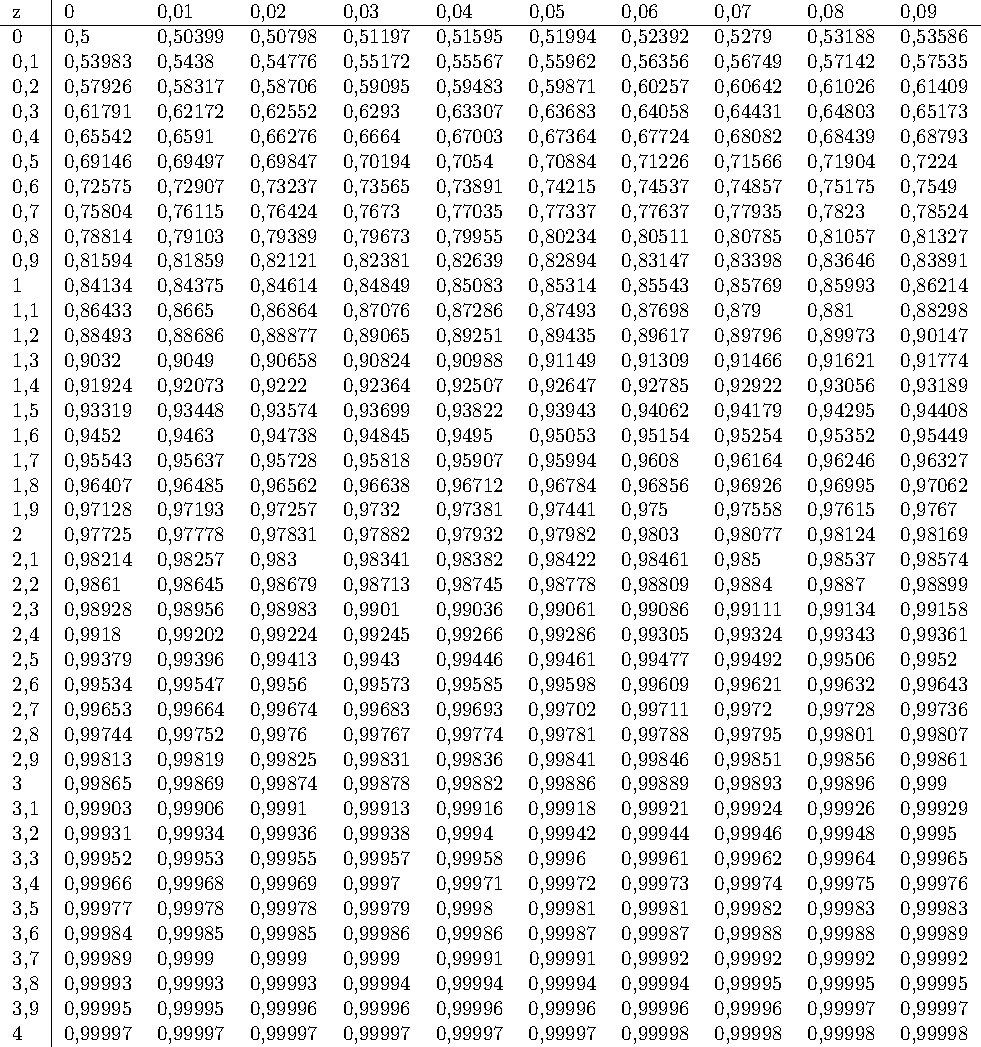
\includepdf[pages=-, scale=0.9]{distribucion_normal.pdf}

%\documentclass{article}
%\usepackage{pgfplots}
%\begin{document}



\begin{tikzpicture}

\pgfmathdeclarefunction{gauss}{2}{%
  \pgfmathparse{1/(#2*sqrt(2*pi))*exp(-((x-#1)^2)/(2*#2^2))}%
}

\begin{axis}[
  no markers, domain=0:10, samples=100,
  axis lines*=left, xlabel=$x$, ylabel=$y$,
  every axis y label/.style={at=(current axis.above origin),anchor=south},
  every axis x label/.style={at=(current axis.right of origin),anchor=west},
  height=5cm, width=12cm,
  xtick={4,6.5}, ytick=\empty,
  enlargelimits=false, clip=false, axis on top,
  grid = major
  ]
  \addplot [fill=cyan!20, draw=none, domain=0:5.96] {gauss(6.5,1)} \closedcycle;
  \addplot [very thick,cyan!50!black] {gauss(4,1)};
  \addplot [very thick,cyan!50!black] {gauss(6.5,1)};


\draw [yshift=-0.6cm, latex-latex](axis cs:4,0) -- node [fill=white] {$1.96\sigma$} (axis cs:5.96,0);
\end{axis}

\end{tikzpicture}

%\end{document}











%\import{probabilidad/}{probabilidad}


\end{multicols*}

\end{document}
